%% =====================================================================
%% COMP 664 course project, Topic 2: plant disease classification
%% Compile with pdfLaTeX (Overleaf default). Main document: main.tex
%% =====================================================================
\documentclass[11pt,letterpaper]{article}
\usepackage[margin=0.8in]{geometry}
\usepackage[T1]{fontenc}
\usepackage{lmodern,microtype,graphicx,booktabs,amsmath,array,caption}
\usepackage[hidelinks]{hyperref}
\usepackage{xurl}
\usepackage{fancyhdr}

%% ---------------------------------------------------------------------
%% EDIT HERE: team information (used on the title block only)
%% ---------------------------------------------------------------------
\newcommand{\TeamMembers}{Zheng Ni, Yuzhi Hu, Enci Zhang, Xinyi Xu} 
%% ---------------------------------------------------------------------

\pagestyle{fancy}\fancyhf{}
\fancyhead[L]{\small COMP 664, Fall 2026}
\fancyhead[R]{\small }
\fancyfoot[C]{\thepage}
\setlength{\headheight}{14pt}
\setlength{\parindent}{0pt}\setlength{\parskip}{5pt}
\captionsetup{font=small,labelfont=bf,hypcap=false}
\makeatletter\let\tableinput\@@input\makeatother
\newcommand{\code}[1]{\texttt{\detokenize{#1}}}

%% Numbers, tables, figures and wording are generated from project/results/ by project/figures.py
\newcommand{\OrdCleanAcc}{97.26}
\newcommand{\OrdCleanAccSD}{0.16}
\newcommand{\OrdCleanFone}{96.32}
\newcommand{\OrdCleanFoneSD}{0.18}
\newcommand{\OrdFieldAcc}{18.78}
\newcommand{\OrdFieldAccSD}{1.10}
\newcommand{\OrdFieldFone}{7.76}
\newcommand{\OrdFieldFoneSD}{0.83}
\newcommand{\AugCleanAcc}{96.66}
\newcommand{\AugCleanAccSD}{0.58}
\newcommand{\AugCleanFone}{95.71}
\newcommand{\AugCleanFoneSD}{0.50}
\newcommand{\AugFieldAcc}{20.13}
\newcommand{\AugFieldAccSD}{0.74}
\newcommand{\AugFieldFone}{9.16}
\newcommand{\AugFieldFoneSD}{0.73}
\newcommand{\DeltaAcc}{+1.35}
\newcommand{\DeltaAccSD}{1.69}
\newcommand{\DeltaFone}{+1.40}
\newcommand{\DeltaFoneSD}{1.31}
\newcommand{\BaseClass}{yellow leaf curl}
\newcommand{\BaseCleanAcc}{32.83}
\newcommand{\BaseCleanFone}{5.49}
\newcommand{\BaseFieldAcc}{10.11}
\newcommand{\BaseFieldFone}{2.04}
\newcommand{\Conclusion}{Strong augmentation improved both field metrics on average, but the paired improvements were not consistent across all three seeds.}
\newcommand{\DemoOrdOne}{late blight}
\newcommand{\DemoAugOne}{late blight}
\newcommand{\DemoOrdTwo}{early blight}
\newcommand{\DemoAugTwo}{late blight}


\begin{document}
\begin{center}
{\Large\bfseries Plant Disease Classification Across\\Clean and Field Images}\par
\vspace{.5em}\TeamMembers
\end{center}

\begin{abstract}
We ask how much a classifier trained on controlled tomato-leaf photographs loses on field images, and whether strong crop and color augmentation reduces that loss. We fine-tune an ImageNet-pretrained MobileNetV3-Small under two matched conditions, ordinary and strong augmentation, using three paired seeds and newly sampled image views in every epoch (six models in total). The official PlantVillage split and all training budgets are fixed, and checkpoint selection uses only PlantVillage validation. Ordinary training reaches $\OrdCleanAcc\pm\OrdCleanAccSD$\% clean accuracy and $\OrdFieldAcc\pm\OrdFieldAccSD$\% field accuracy. Strong augmentation reaches $\AugCleanAcc\pm\AugCleanAccSD$\% and $\AugFieldAcc\pm\AugFieldAccSD$\%, respectively (mean $\pm$ sample SD over seeds). The mean paired field changes are $\DeltaAcc$ percentage points in accuracy and $\DeltaFone$ in macro-F1. \Conclusion\ Absolute field performance remains low: a training-only majority-class classifier reaches \BaseFieldAcc\% field accuracy. An earlier single-seed pilot is summarized in Appendix~\ref{app:pilot}. Code, the processed file list, checkpoints, per-image predictions, audits, and an executed Notebook accompany the report.
\end{abstract}

%% ---------------------------------------------------------------------
\section{Question and comparison}
A classifier can perform well on controlled leaf photographs yet fail under different backgrounds, lighting, scales, and viewpoints. Our question is: How large is the clean-to-field gap, and can crop and color augmentation reduce it? We use one backbone and compare two training procedures, rather than searching across architectures. Each input is one RGB photograph; the target is one of nine shared tomato labels.

The main experiment is a three-seed comparison of ordinary and strong-augmentation training with fresh views in every epoch. Both conditions use the same examples, trainable blocks, optimizer settings, batch size, and eight-epoch budget. All six checkpoint choices are finalized before either test set is scored. An earlier single-seed pilot with two fixed views per image is summarized in Appendix~\ref{app:pilot}; it is not part of the main comparison.

\begin{center}
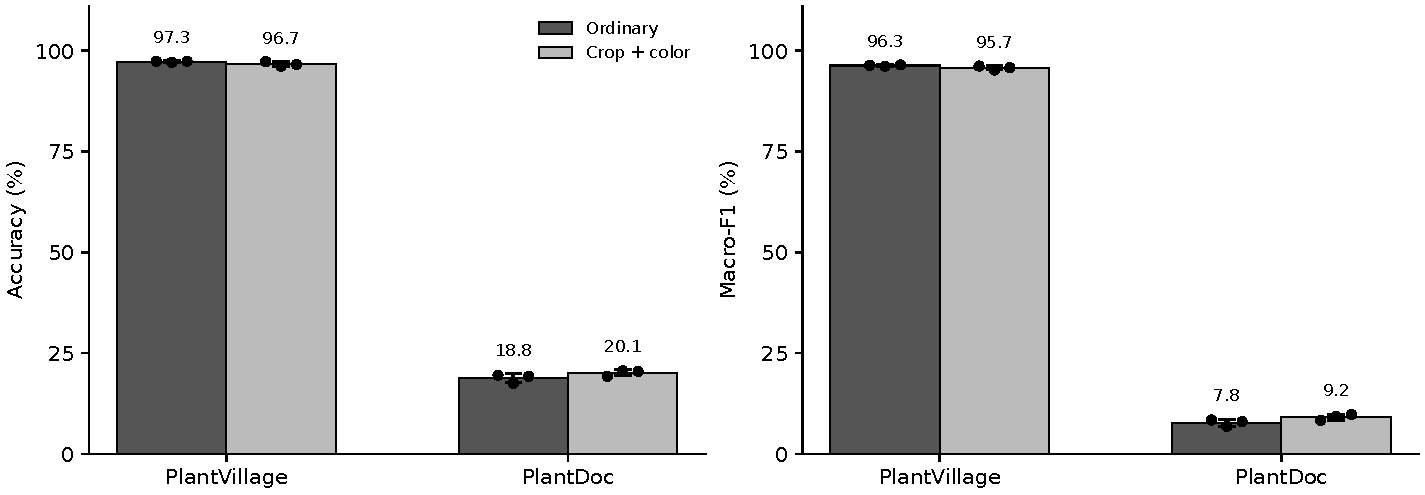
\includegraphics[width=.95\linewidth]{figures/performance.pdf}
\captionof{figure}{Performance of the six models. Bars show the mean of three seeds; error bars show sample SD, and dots show individual runs. All runs use the same 3,351 clean and 742 field test images.}
\end{center}

%% ---------------------------------------------------------------------
\section{Data and split integrity}
PlantVillage provides controlled leaf photographs \cite{pv}; Cropped-PlantDoc provides the external classification images \cite{pd}. We use the nine-class mapping in the course specification and exclude PlantVillage target spot. Folder names are case-folded and stripped of non-alphanumeric characters before mapping. Exact names and class indices are saved in \code{project/results/class_mapping.csv}, and the processed file list (path, split, label, leaf group, and SHA-256 of every image) in \code{project/results/manifest.csv}, submitted with the code.

We preserve the official leaf-grouped PlantVillage color train/test lists. Within its original training partition, 15\% of documented leaf groups per class (rounded, split seed 664) enter validation. This data split is identical across training seeds. Images without a documented leaf ID stay in training. PlantDoc's original train and test folders are pooled \emph{only} as the external test: no PlantDoc image enters optimization or checkpoint selection.

\begin{center}\small
\begin{tabular}{lrrrr}\toprule
Class & Train & Validation & Clean test & Field test\\\midrule
\tableinput figures/counts.tex
\midrule Total & 12,036 & 1,364 & 3,351 & 742\\\bottomrule
\end{tabular}
\captionof{table}{The audited data split, identical in all six runs.}
\end{center}

\textbf{Incomplete group metadata.} Exactly 4,280 training and 1,060 clean-test images lack documented leaf IDs. No retained \emph{documented} leaf group crosses splits, but unknown identities prevent a complete same-leaf independence guarantee. Mosaic virus has no documented training leaf groups and therefore zero validation examples. Selection uses the eight supported validation classes; training and both tests cover all nine. We do not create potentially leaking image-level validation samples to fill this missing class.

\textbf{Duplicate audit.} SHA-256 checks remove five source-training entries with copies in held-out splits. Among 746 mapped PlantDoc entries, two redundant same-label copies and both copies of one contradictory-label image are removed, leaving 742 byte-unique entries. These checks do not rule out visually similar crops, recompressed images, or near-duplicates. The two spider-mite examples are visually related multi-panel illustrations, so their independence and representativeness are especially uncertain. Reconstruction of the file lists from pinned upstream revisions is described in Appendix~\ref{app:repro}.

%% ---------------------------------------------------------------------
\section{Training protocol with fresh views}
We replace the ImageNet MobileNetV3-Small output layer with nine logits \cite{mobile}. The prefix is frozen in evaluation mode; the last inverted residual block, final convolution, and classifier are trained (950,617 of 1,527,081 parameters). Within each seed, both conditions begin from the same complete state and receive exactly the same shuffled image indices in every epoch. Freezing the early layers keeps six runs affordable on one GPU and holds the ImageNet features fixed, so the two conditions differ only in the training views; full fine-tuning was not tested. The experiment isolates the training procedure; it does not compare backbones.

\begin{center}\small
\begin{tabular}{p{.27\linewidth}p{.65\linewidth}}\toprule
Setting & Prespecified value\\\midrule
Seeds and budget & 664, 665, 666; two conditions each; 8 epochs, batch 96\\
Optimization & Cross-entropy; AdamW, learning rate $5\times10^{-4}$, weight decay $10^{-4}$\\
Input and normalization & RGB, $128\times128$; ImageNet channel mean and standard deviation\\
Ordinary & Resize, horizontal flip with probability 0.5\\
Strong & Additional random crop (area .55--1.0, log-uniform aspect ratio .8--1.25); brightness/contrast/saturation jitter .35 and hue jitter .07\\
Image exposure & 12,036 images per epoch; 1,008 optimizer steps and 96,288 presentations per model\\
Selection & First epoch maximizing source-validation supported-class macro-F1\\
Execution & One RTX 5070 Ti Laptop GPU; PyTorch 2.7.1+cu128, torchvision 0.22.1+cu128; deterministic algorithms; TF32 disabled\\\bottomrule
\end{tabular}
\captionof{table}{Matched settings for the six models. No target-domain adaptation or architecture search is performed.}
\end{center}

\textbf{Fresh views, not cached random transformations.} We cache only deterministic EXIF-corrected RGB resizing as uint8 pixels. Each image receives a newly sampled PIL transformation in each epoch. A local RNG keyed by training seed, epoch, and image index makes the views reproducible independently of thread scheduling. Ordinary flip draws are fresh even though only two flipped/unflipped outcomes are possible. Strong crops and color factors are redrawn each epoch. Frozen-prefix activations are computed afresh per batch, converted to float16, then returned to float32 for the trainable blocks; they are never reused across epochs.

\textbf{Recorded evidence.} Each run logs loss, validation scores, sample-order and initialization hashes, and selected weights; an aggregate audit checks the pairing and a checkpoint lock written before test evaluation (Appendix~\ref{app:repro}). Total exposure is 577,728 image presentations and 6,048 optimizer steps.

\begin{center}
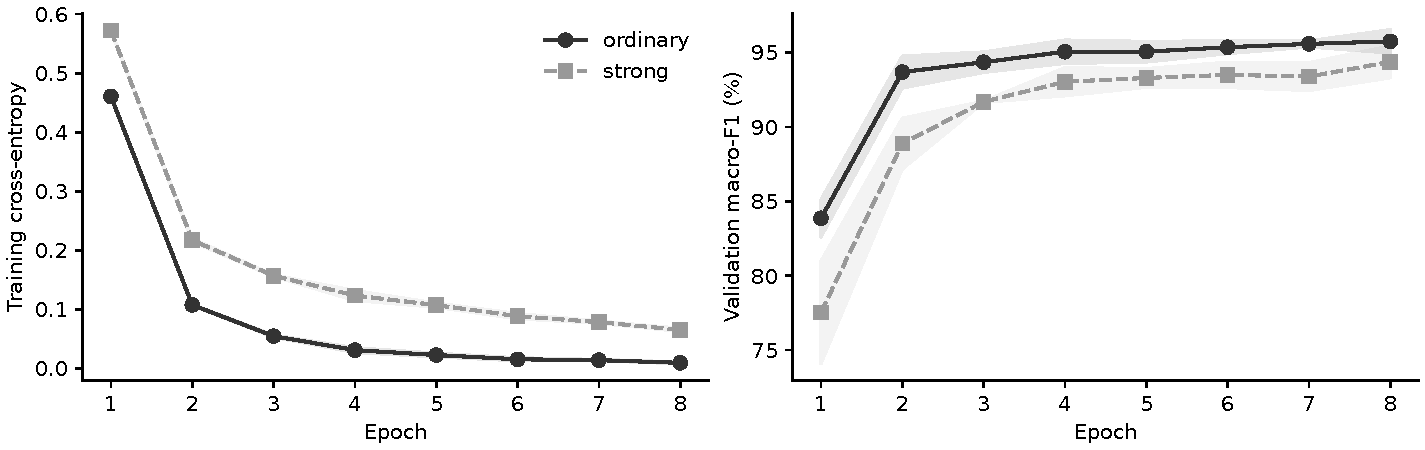
\includegraphics[width=.95\linewidth]{figures/history.pdf}
\captionof{figure}{Mean training loss and supported-class validation macro-F1 over three seeds; shading shows sample SD. Epoch selection is performed separately for each model.}
\end{center}

%% ---------------------------------------------------------------------
\section{Overall results and seed variability}
Accuracy is the correct-prediction fraction. Test macro-F1 averages all nine class F1 scores equally, using zero for an undefined class score. The clean-to-field gap is the clean metric minus the field metric, in percentage points (pp). A smaller gap alone does not establish improved field performance.

\begin{center}\small
\begin{tabular}{lrrrr}\toprule
 & \multicolumn{2}{c}{Accuracy (\%)} & \multicolumn{2}{c}{Macro-F1 (\%)}\\
Training & Clean & Field & Clean & Field\\\midrule
\tableinput figures/summary.tex
\bottomrule\end{tabular}
\captionof{table}{Results of the three-seed experiment, mean $\pm$ sample SD over the three paired seeds. These are three fits on the same test collections, not three independent datasets.}
\end{center}

\begin{center}\small
\begin{tabular}{rlrrrrr}\toprule
 & & Selected & \multicolumn{2}{c}{Accuracy (\%)} & \multicolumn{2}{c}{Macro-F1 (\%)}\\
Seed & Training & epoch & Clean & Field & Clean & Field\\\midrule
\tableinput figures/seeds.tex
\bottomrule\end{tabular}
\captionof{table}{Every run, without selection by field performance. Seed 664 is fixed as the illustrative checkpoint pair for figures and demonstrations.}
\end{center}

\begin{center}\small
\begin{tabular}{rrr}\toprule
Seed & Field accuracy change (pp) & Field macro-F1 change (pp)\\\midrule
\tableinput figures/deltas.tex
\bottomrule\end{tabular}
\captionof{table}{Paired strong-minus-ordinary changes. Their mean $\pm$ SD is $\DeltaAcc\pm\DeltaAccSD$ pp for accuracy and $\DeltaFone\pm\DeltaFoneSD$ pp for macro-F1.}
\end{center}

\Conclusion\ Three seeds expose training variability but remain too few for a strong claim of universal benefit or equivalence. Per-seed class-stratified paired bootstrap intervals are also supplied; they condition on each fitted pair and observed field images, and do not replace seed variability.

\textbf{Reference floor.} A training-only majority-class classifier reaches \BaseFieldAcc\% field accuracy and \BaseFieldFone\% field macro-F1 (Section~\ref{sec:baseline}). Both conditions exceed this floor but remain far below their clean-test performance.

%% ---------------------------------------------------------------------
\section{Per-class gaps and errors}
\begin{center}\begin{minipage}{\linewidth}\centering\small
\begin{tabular}{lr rrr rrr}\toprule
 & Field & \multicolumn{3}{c}{Ordinary recall (\%)} & \multicolumn{3}{c}{Strong recall (\%)}\\
Class & $n$ & Clean & Field & Gap & Clean & Field & Gap\\\midrule
\tableinput figures/recall.tex
\bottomrule\end{tabular}
\captionof{table}{Per-class recall averaged over three seeds. Clean is the in-domain (PlantVillage) test, Field the cross-domain (PlantDoc) test; the gap is clean minus field in pp, computed from unrounded means.}
\end{minipage}\end{center}

\begin{center}\begin{minipage}{\linewidth}\centering\small
\begin{tabular}{lr rrr rrr}\toprule
 & Field & \multicolumn{3}{c}{Ordinary F1 (\%)} & \multicolumn{3}{c}{Strong F1 (\%)}\\
Class & $n$ & Clean & Field & Gap & Clean & Field & Gap\\\midrule
\tableinput figures/f1.tex
\bottomrule\end{tabular}
\captionof{table}{Per-class F1 averaged over three seeds, with the clean-minus-field gap in pp. Unlike recall, F1 also penalizes predicting a class too often, so late blight has high field recall but low field F1. Per-seed values and SDs are in \code{project/results/per_seed_class_gaps.csv}.}
\end{minipage}\end{center}

Ordinary training most often predicted late blight, assigning that label to 540.0 of 742 field images on average (SD 85.8); its true support was 111. Strong training most often predicted late blight, assigning that label to 543.7 of 742 field images on average (SD 56.3); its true support was 111. The largest signed mean class-recall change was +10.7 pp for septoria, and the smallest was -8.3 pp for early blight.


\begin{center}
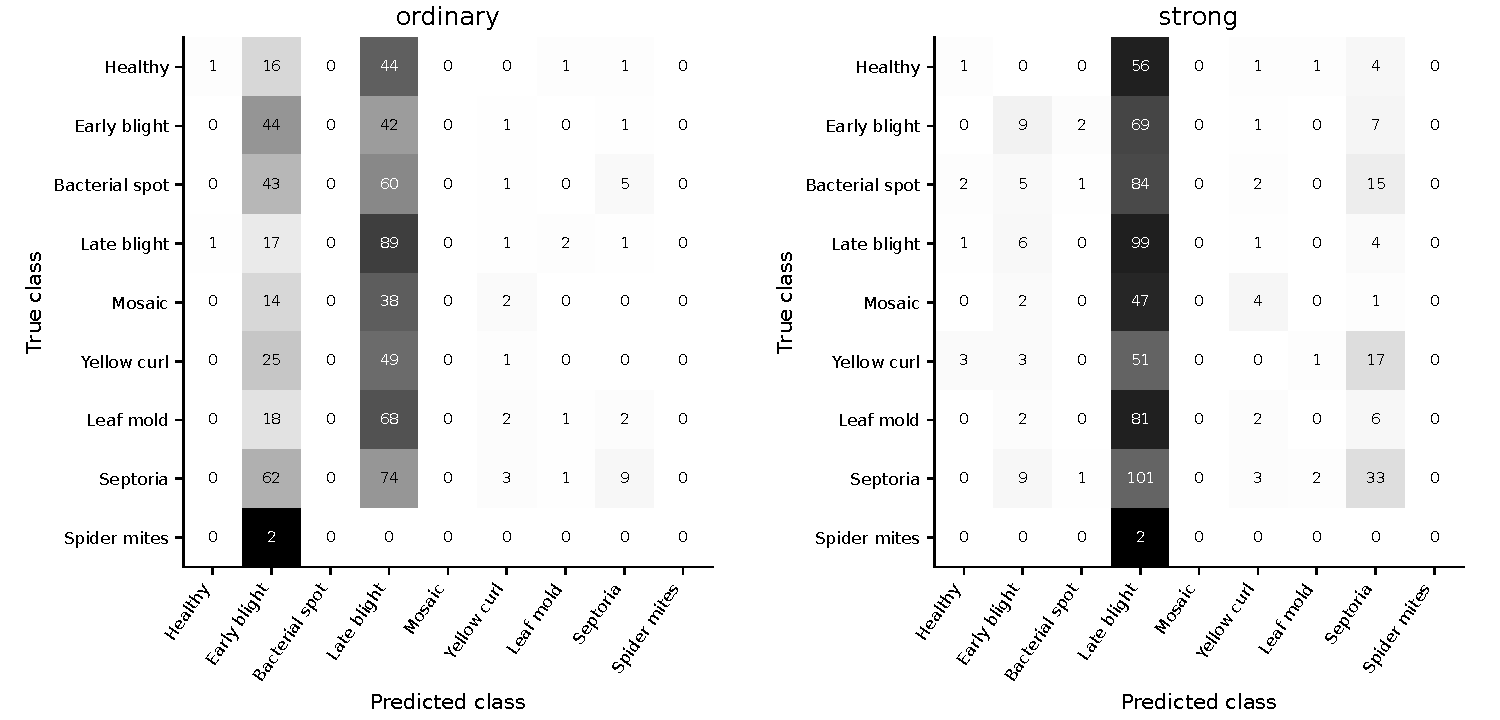
\includegraphics[width=.94\linewidth]{figures/confusions.pdf}
\captionof{figure}{Field confusion counts for the prespecified illustrative seed 664. Rows are true classes; columns are predictions. Grayscale uses the fraction within each true class. This pair was not chosen for its field score.}
\end{center}

High recall for a frequently predicted label can coexist with poor precision and zero recall for other labels. Macro-F1 exposes this concentration. The two spider-mite entries receive the same macro-F1 weight as 149 Septoria images; one changed spider-mite prediction shifts that run's class recall by 50 pp. Averaging seeds does not create additional independent spider-mite examples.

%% ---------------------------------------------------------------------
\section{Baseline, confidence, and example photographs}\label{sec:baseline}
\textbf{Training-only majority-class baseline.} A constant classifier chosen by the most common \emph{source training} label (\BaseClass) achieves \BaseCleanAcc\% clean and \BaseFieldAcc\% field accuracy, with macro-F1 \BaseCleanFone\% and \BaseFieldFone\%. No field label is used to choose this baseline. Exceeding it does not imply useful diagnostic performance.

\begin{center}\small
\begin{tabular}{rlrrr}\toprule
Seed & Training & High-confidence $n$ & Correct & Accuracy (\%)\\\midrule
\tableinput figures/confidence.tex
\bottomrule\end{tabular}
\captionof{table}{Field predictions with maximum softmax $\geq0.9$. These uncalibrated scores must not be interpreted as reliable disease probabilities.}
\end{center}

\begin{center}
\begin{minipage}{.47\linewidth}\centering
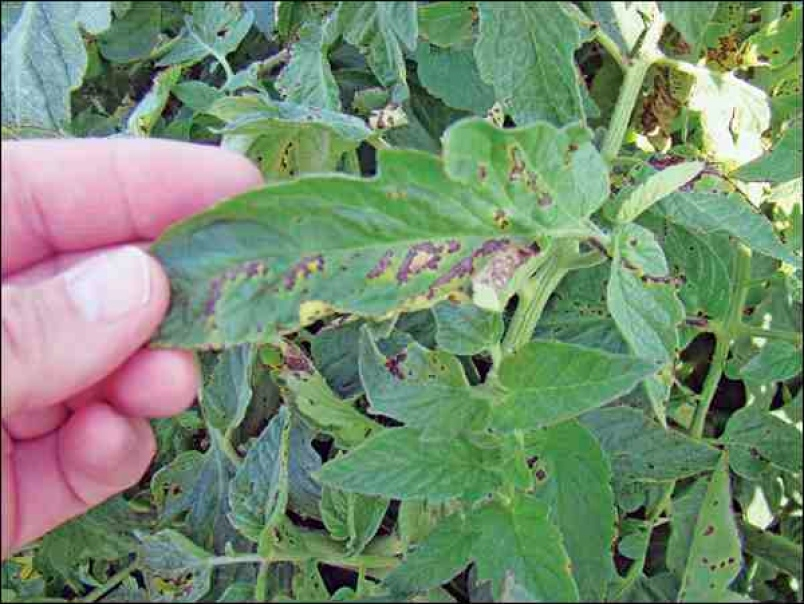
\includegraphics[height=1.8in,width=.95\linewidth,keepaspectratio]{figures/examples/field.jpg}\\
\small Label: early blight.\\Ordinary: \DemoOrdOne.\\Strong: \DemoAugOne.
\end{minipage}\hfill
\begin{minipage}{.47\linewidth}\centering
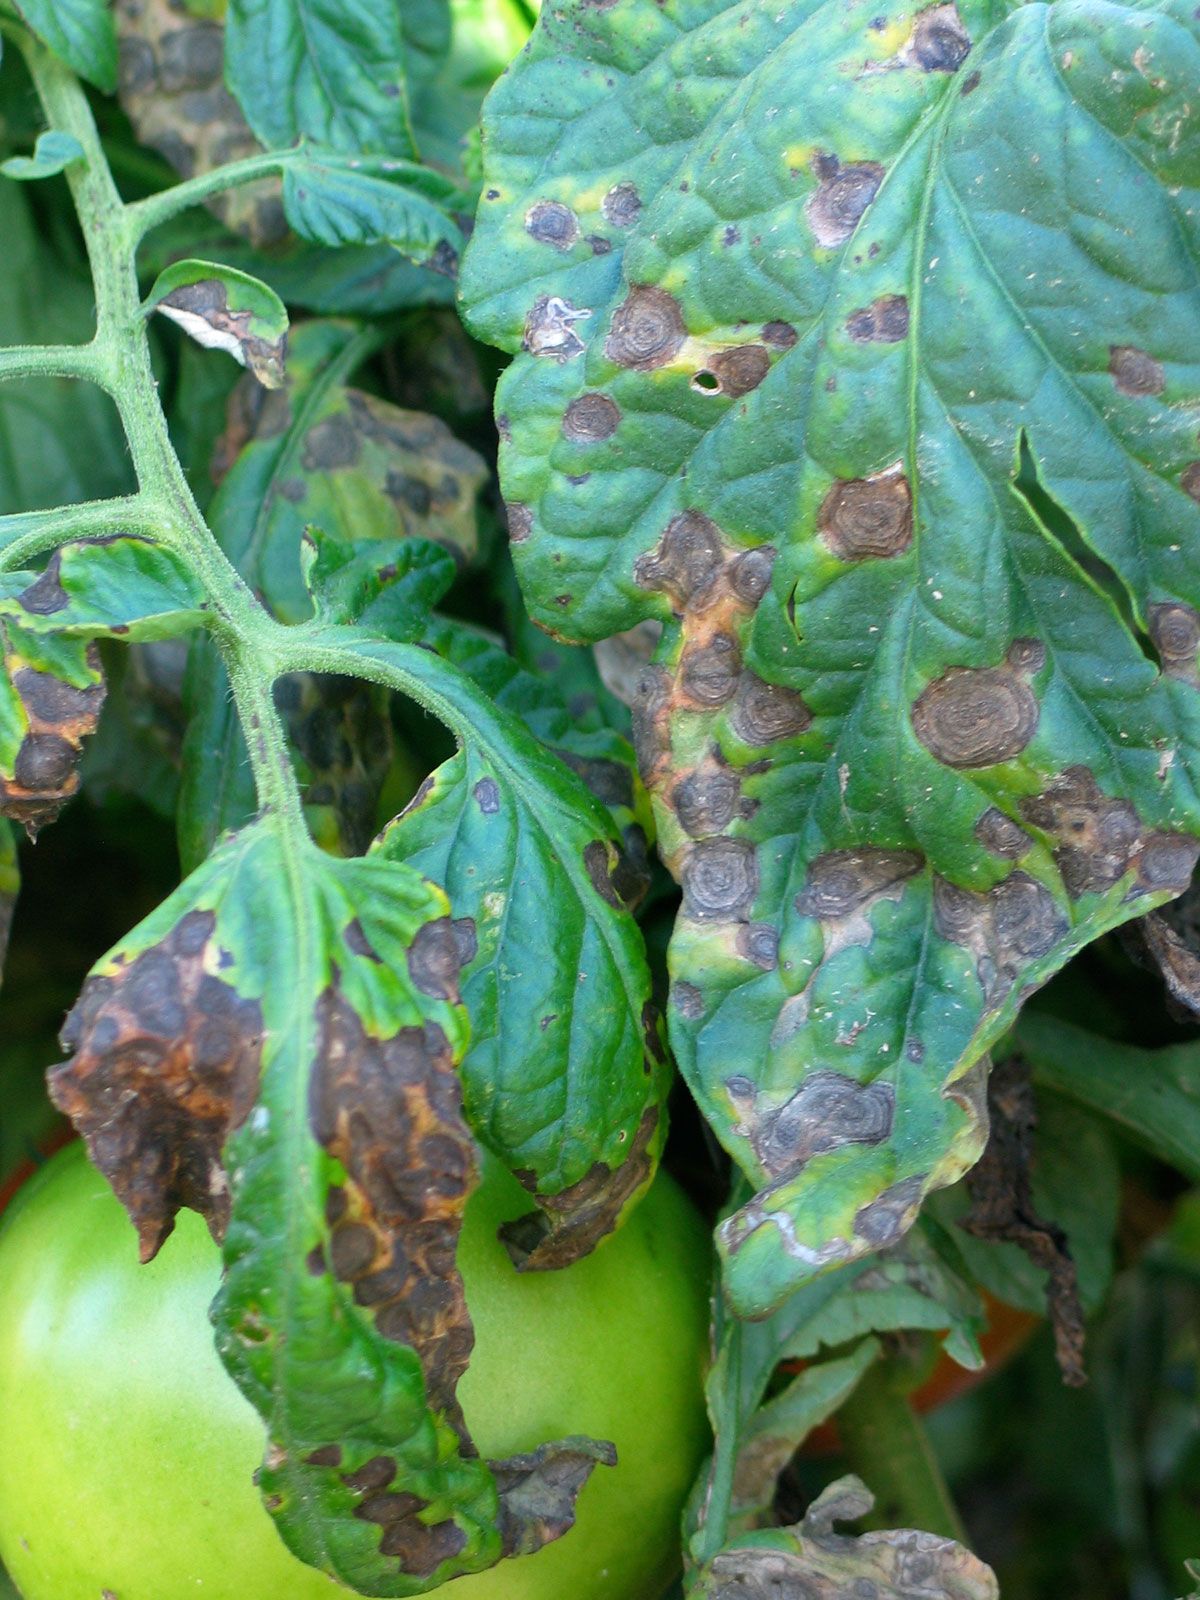
\includegraphics[height=1.8in,width=.95\linewidth,keepaspectratio]{figures/examples/field_second.jpg}\\
\small Label: early blight.\\Ordinary: \DemoOrdTwo.\\Strong: \DemoAugTwo.
\end{minipage}
\captionof{figure}{Two fixed demonstration photographs, scored by the seed-664 pair. They were selected during the earlier pilot analysis, before the three-seed runs, and do not estimate typical performance. Exact paths and credits appear in \code{project/examples/credits.csv}.\label{fig:examples}}
\end{center}

\textbf{Reading the examples.} Individual corrections or regressions do not determine the main conclusion. We use all test images and all prespecified seeds for that comparison. The executed Notebook loads the actual checkpoints for offline inference, checks the example hashes, and compares the predictions with the saved full-test evidence.

%% ---------------------------------------------------------------------
\section{Limitations and conclusion}
\Conclusion\ This applies to the specified backbone, partial fine-tuning, resolution, budget, transformations, and collections. It does not establish the behavior of all augmentation strategies or a reliable field diagnostic system.

\textbf{Absolute performance.} Field accuracy of about 19--20\% is only about 9--10 pp above the \BaseFieldAcc\% majority-class floor, and most field images are assigned to one label (late blight). We did not test larger backbones, higher input resolution, or full fine-tuning, so the study speaks to the effect of augmentation in this training setup rather than to the best achievable field accuracy.

\textbf{Data limits.} Mosaic virus still lacks validation support. Unknown leaf IDs and near-duplicates prevent a full independence guarantee. PlantDoc is an internet-collected cropped-image benchmark with ambiguous examples, not a prospective collection of independently diagnosed farm leaves. Its two spider-mite entries provide weak class evidence. Three seeds describe limited optimization variation, not variation across farms, seasons, or dataset construction.

\textbf{Exploratory status.} The three-seed experiment was designed after inspecting the pilot's field results (Appendix~\ref{app:pilot}). Field labels never enter optimization or checkpoint selection, but the benchmark was already examined: this is exploratory follow-up evidence, not a pristine confirmatory external test. A stronger study would predefine a new target-development/test separation and evaluate on an independent field collection. Target-domain fine-tuning must use its own development subset.

%% ---------------------------------------------------------------------
\section{Reproducibility}
All code and results are in the submitted \code{project/} folder, and the paths below are relative to it: \code{data.py} (download, mapping, split), \code{train.py} (the six training runs and test evaluation), \code{analysis.py} (metrics, independent audit, three-seed summary), \code{figures.py} (report figures and tables), \code{replay.py} (raw-image replay), and \code{demo.py}. \code{results/} holds the frozen protocol, timestamped events, selected weights, per-epoch histories, per-image probabilities, class metrics, and audits; \code{selection_locked.json} records all six checkpoint hashes before test scoring. The executed Notebook recomputes the statistics and runs the checkpoints on example photographs without retraining. Provenance details and commands are in Appendix~\ref{app:repro}.

\begin{thebibliography}{9}\small
\bibitem{pv} S. P. Mohanty, D. P. Hughes, and M. Salath\'e. Using Deep Learning for Image-Based Plant Disease Detection. \emph{Frontiers in Plant Science}, 7:1419, 2016. \url{https://doi.org/10.3389/fpls.2016.01419}. Data and leaf metadata: \url{https://github.com/spMohanty/PlantVillage-Dataset}; official split lists: \url{https://huggingface.co/datasets/mohanty/PlantVillage/tree/main/splits}.
\bibitem{pd} D. Singh et al. PlantDoc: A Dataset for Visual Plant Disease Detection. \emph{CoDS-COMAD}, 2020. \url{https://doi.org/10.1145/3371158.3371196}. Cropped classification data: \url{https://github.com/pratikkayal/PlantDoc-Dataset}, CC BY 4.0.
\bibitem{mobile} A. Howard et al. Searching for MobileNetV3. \emph{ICCV}, 2019. \url{https://arxiv.org/abs/1905.02244}. Three-seed runs: torchvision 0.22.1, \code{IMAGENET1K_V1}; pilot: torchvision 0.20.1 with the same ImageNet initialization.
\end{thebibliography}

%% ---------------------------------------------------------------------
\appendix
\section{Earlier single-seed pilot}\label{app:pilot}
Before the three-seed study, a pilot trained ordinary and strong-augmentation models with two fixed augmented views per image. It used one seed, PyTorch 2.5.1 on CPU, and cached prefix activations. It achieved 97.25\% clean and 19.54\% field accuracy with ordinary training, and 96.09\% and 18.73\% with strong augmentation (field macro-F1 8.67\% and 8.57\%).

The three-seed runs change view refresh, RNG implementation, data streaming, and execution environment. A difference from the pilot therefore cannot be attributed purely to fresh augmentation; the controlled comparison is ordinary versus strong \emph{within} the matched three-seed protocol. The two demonstration photographs in Figure~\ref{fig:examples} were chosen during the pilot analysis and were not reselected afterwards.

The pilot's weights, predictions, and code are not part of the final repository; they remain in its git history (commit \code{adb96c0}). Replaying both pilot checkpoints on all 4,093 raw test images reproduced all 8,186 labels (probability differences below 0.000260), which confirms inference, not the pilot's training history.

\section{Reproducibility and provenance}\label{app:repro}
\textbf{Data reconstruction.} Fixed upstream revisions regenerate the manifest, exclusions, and class mapping byte for byte (\code{data.py}). Deterministic image decoding checks every raw file against its recorded SHA-256. Portable disk names encode Windows-invalid characters while the manifest keeps the original paths. These are integrity checks, not proof that every label is biologically correct. Raw data are not bundled; the pinned archives need about 3.5 GB.

\textbf{Run records.} Each run logs loss, validation scores, optimizer steps, sample-order and initialization hashes, selected weights, and completion records. \code{analysis.py} checks equal initialization and order within each pair, the training budgets, unchanged frozen-prefix parameters, all 48 epochs, and that every checkpoint still matches its hash locked before test evaluation; it also recomputes every metric from the per-image predictions.

\textbf{Independent replay.} After training, all six models were replayed on the raw test images: all 24,558 predicted labels matched the saved predictions (maximum probability difference 0.0003113); see \code{results/replay_verification.json}.

\textbf{Code consolidation.} The models were trained by \code{experiment_fresh.py} (SHA-256 recorded in \code{results/protocol.json}), kept in commit \code{adb96c0}. The code was later consolidated into the files above. On a synthetic dataset, the old and new code produced identical downloads and manifests, bit-identical checkpoints, identical training histories, byte-identical predictions and metric tables, and identical replay results; on the saved results, \code{analysis.py} and \code{figures.py} reproduce every table, macro, and figure exactly.

\textbf{Commands} (run from \code{project/}):
\begin{small}
\begin{verbatim}
python analysis.py --results results    # recompute and audit every table
python -m unittest discover -s tests -v
python demo.py examples/field.jpg
python data.py --data data              # raw data, ~3.5 GB
python train.py --data data --out rerun --device cuda
python replay.py --data data --seed-dir results/seed_664
\end{verbatim}
\end{small}
Training used PyTorch 2.7.1+cu128 on one GPU (\code{requirements-train.txt}); the Notebook, demo, analysis, and tests use PyTorch 2.5.1 on CPU (\code{requirements.txt}).
\end{document}
